\section{Event Selection}

This section explains the procedure to improve the identification of the particles, corrections to the event and cuts to the analysis. 

\subsection{Selection of the Beam Photon}

A typical g12 data event has multiple bremsstrahlung photons recorded as the incident beam. The multiple beam photon arises from 2.004 beam bunching spacing of the electrons in the storage ring. These electrons gives the bremsstrahlung photons in the radiator and creates multiple hits in the trigger and thereby satisfying trigger logic to record them. All the  photons which falls within the timing window of $\mid$Tagger Time - StartTime$\mid$ $\leq$ 1.002 ns are considered as an individual event.

\subsection{G12 Corrections}
\label{Cor}
The G12 Corrections were derived from the exclusive $\pi^{+}$, $\pi^{-}$ and proton reaction. We used the following corrections in the analysis ~\cite{G12_AN}:
    
\begin {itemize}
\item Beam Energy Correction : Is a correction to the incident beam photon energy and dependent on the Run number of the event. This correction is only applicable data and not to the simulated events.
\item Removal of bad TOF paddle : This correction takes the Sector number and Paddle number as input. We used the correction to remove only those paddles that shows a significant drift on the resolutions of particle.   
\item  Geometric Fiducial Cut : This cut removes the dead part of the detector from the $\theta-\phi$ map of the particle. We used it with the "nominal" option. 
\end {itemize}

\subsection{Kinematic Fitting}
\label{KF}
Kinematic fitter is a useful tool often used to get rid of unwanted background from signal channels and helps to improve the signal to background ratio.  Any measurement with a tool comes with an error, and it can be represented as a vector  $\vec{\eta}$. We can also define the measurement as 
\\ $\vec{\eta}$ =  $\vec{y}$. +  $\vec{\epsilon}$.\\
Where the $\vec{y}$ and $\vec{\epsilon}$ denotes the actual value of the measurement without error and $\vec{\epsilon}$ is the error associated with the measurement. The kinematic information of a physics channel along with the constrains imposed allows the fitter to calculate the probability and $\chi^{2}$ of each event using Lagrange multipliers to perform a least-squares fit. The CLAS g12 Kinematic fitter takes the ``TBER (Track Based Error)" matrix, vertex of information and four-momentum of all particles as input, and returns Pull probabilities and $\chi^{2}$ for each events. The Pull probabilities when fitted with Guassian, its mean and $\sigma$ decides the quality of the covariance matrix and kinematic fit. In the ideal case of gaussian fitted to the Pulls of the particles should have  zero mean and $\sigma$ of one, which ensures that the fitter correctly calculates covariance matrix error. 
  
\begin{figure}[ht!]
\centerline{
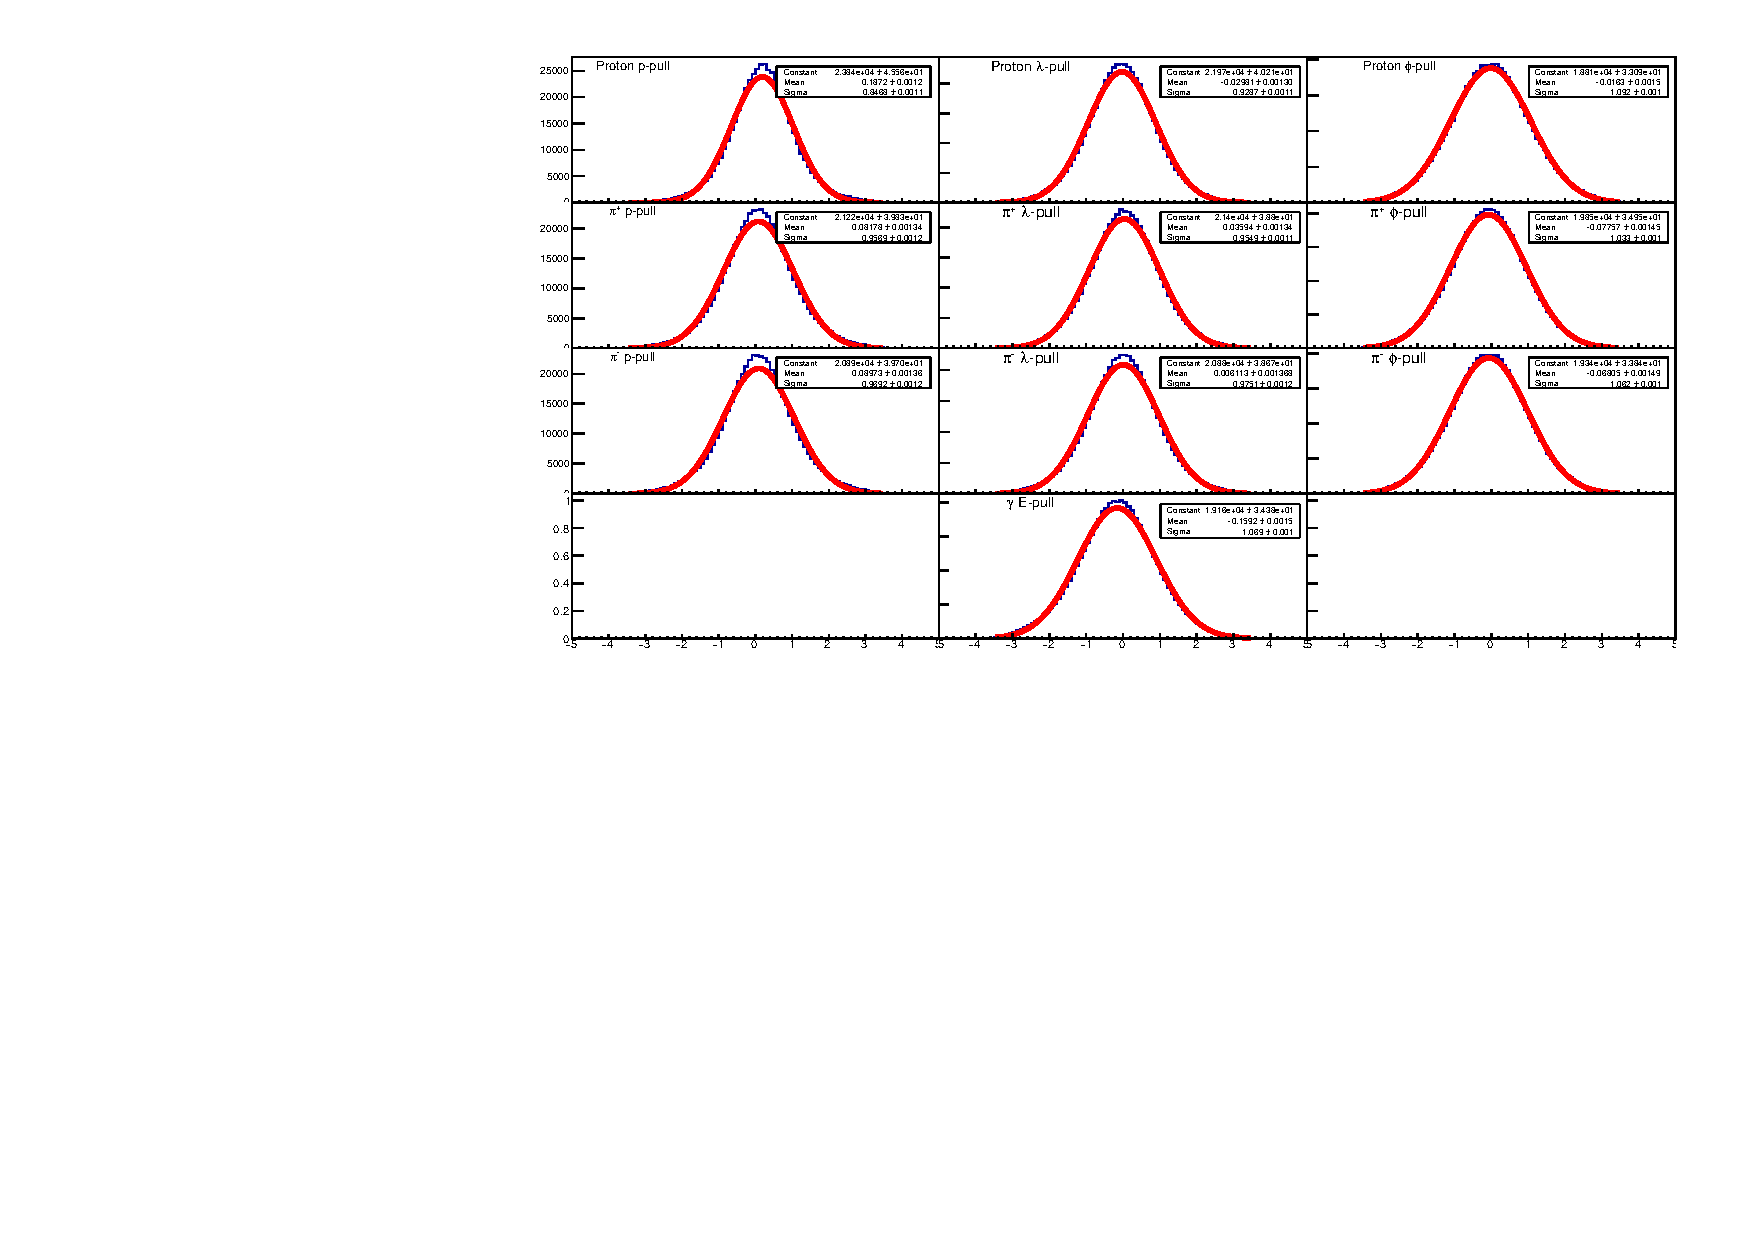
\includegraphics[width=12cm,height=10cm]{Pulls_nothing.pdf}}
\caption{The Pull distributions for a (4-C) kinematic fit to $\gamma$ p $\rightarrow$ $\pi^{+}$ $\pi^{-}$ p from g12 data with run 56655 after a 1$\%$ Pull probability cut.}
\label{Fig3}
\end{figure}

\begin{figure}[ht!]
\centerline{
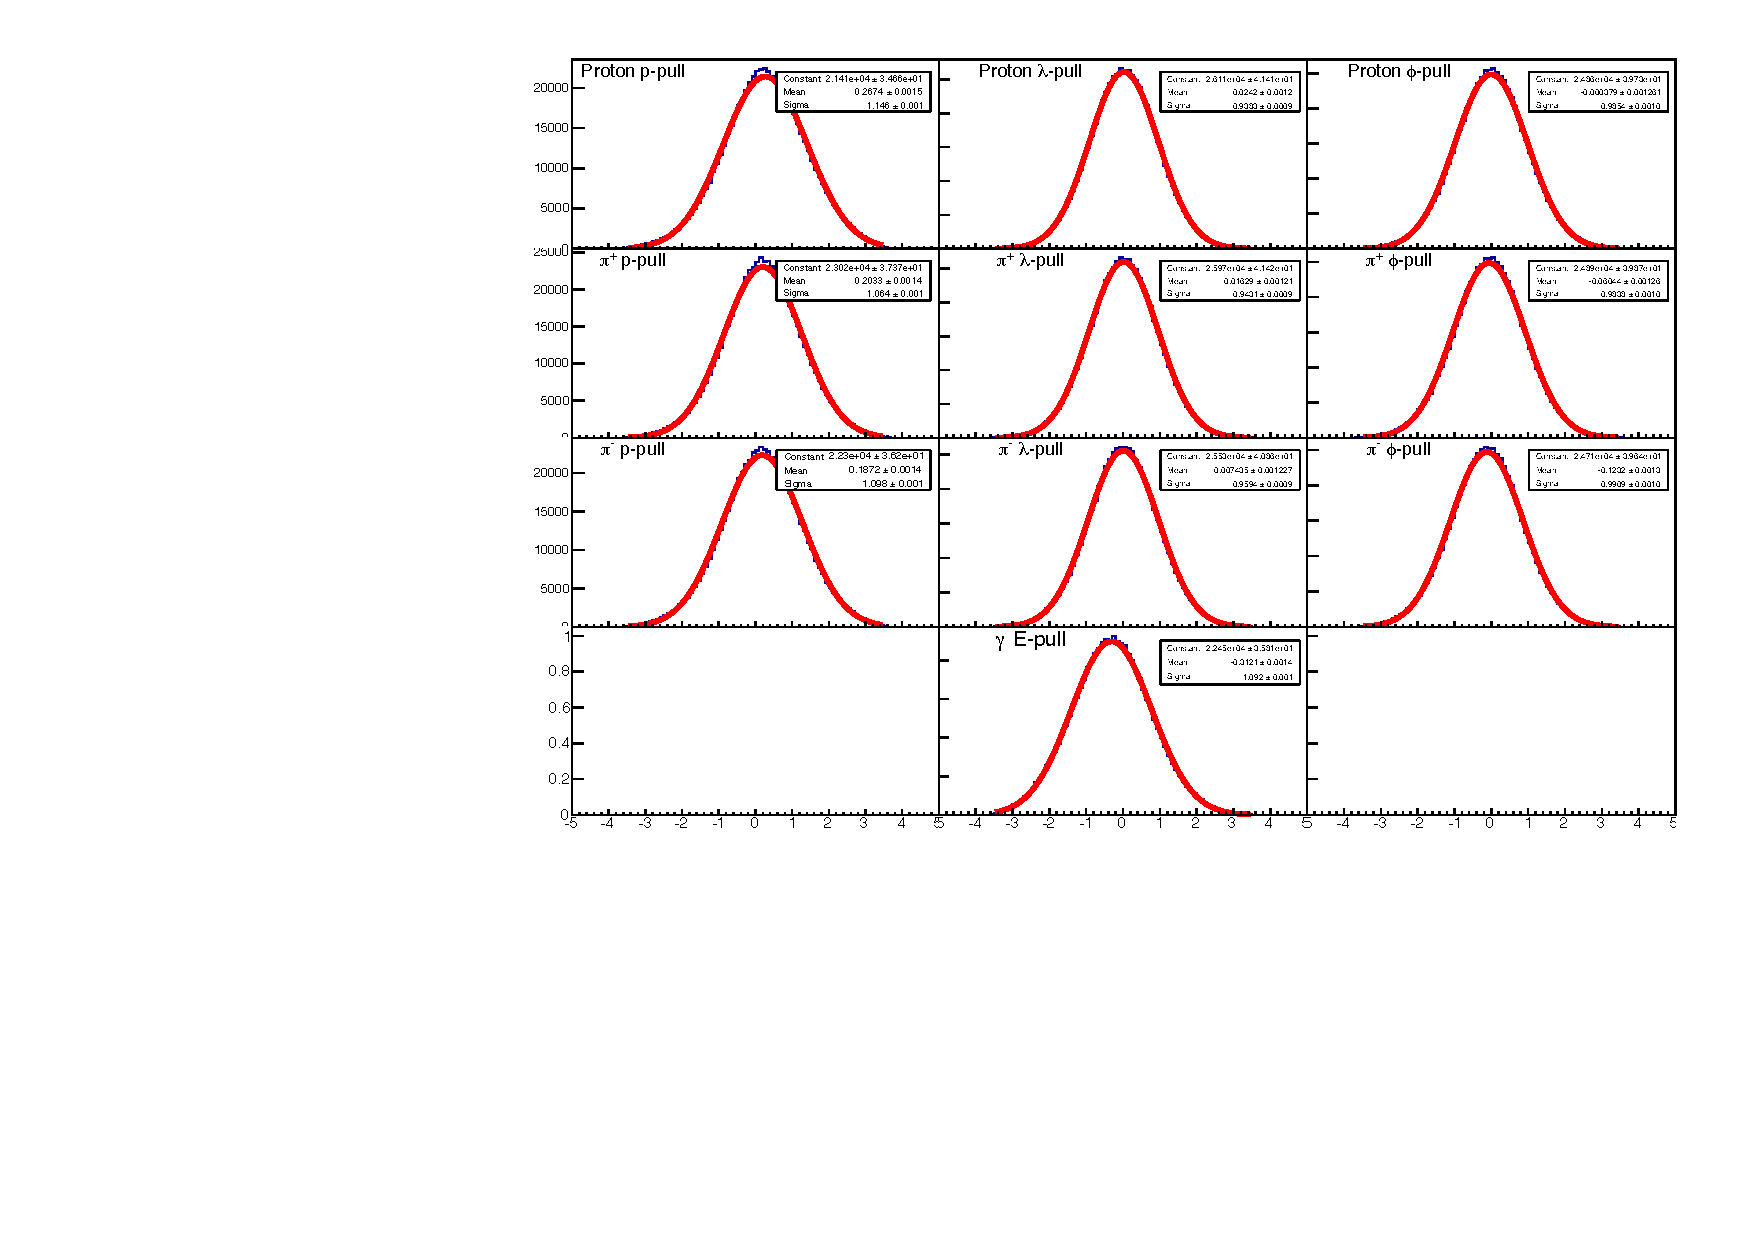
\includegraphics[width=12cm,height=10cm]{SIM_Pulls_nothing.pdf}}
\caption{The Pull distributions for a (4-C) kinematic fit to $\gamma$ p $\rightarrow$ $\pi^{+}$ $\pi^{-}$ p from g12 simulation after a 1$\%$ Pull probability cut.}
\label{Fig4}
\end{figure}
  
The CLAS g12 Kinematic fitter is tuned for 4C constrained reaction,

\begin{eqnarray*}
\gamma p \rightarrow \pi^{+} \pi^{-} p.
\end{eqnarray*}\\
\noindent
The tuning were done for $\pi^{+}$ $\pi^{-}$ and p individually. To check the quality of covariance matrix the mean and sigma of the tuned pulls of the particles $\pi^{+}$, $\pi^{-}$ and p from the reaction hypothesis for the data with run 56655 and simulation after a 1$\%$ pull probability cut is listed in the Table.~\ref{tab2}.

\begin{table}
\centering
\begin{subtable}{.5\textwidth}
\centering
\caption{ }
\begin{tabular}{ |c|c|c| }
\hline
                                                &$\mu$   &$\sigma$ \\
                               \hline
Proton p-pull                            & 0.187  & 0.846  \\
\hline
Proton $\lambda$-pull                      & -0.029 & 0.928  \\
\hline
Proton $\phi$-pull                         & -0.016 & 1.092  \\
\hline
$\pi^{+}$ p-pull        & 0.081  & 0.957  \\
\hline
$\pi^{+}$ $\lambda$-pull & 0.035  & 0.954  \\
\hline
$\pi^{-}$ $\phi$-pull    & -0.077 & 1.033  \\
\hline
$\pi^{-}$ p-pull        & 0.089  & 0.969  \\
\hline
$\pi^{-}$ $\lambda$-pull & 0.006  & 0.975  \\
\hline
$\pi^{-}$ $\phi$-pull    & -0.068 & 1.062  \\
\hline
$\gamma$ E-pull   & -0.159 & 1.069 \\
\hline
\end{tabular}
\end{subtable}%
\begin{subtable}{.5\textwidth}
\centering
\caption{ }
\begin{tabular}{ |c|c|c| }
\hline
                                         &$\mu$   &$\sigma$ \\ \hline
Proton p-pull                             & 0.267  & 1.146  \\
\hline
Proton $\lambda$-pull                  & 0.024  & 0.938  \\
\hline
Proton $\phi$-pull                         & -0.000 & 0.985  \\
\hline
$\pi^{+}$ p-pull        & 0.203  & 1.064  \\
\hline
$\pi^{+}$ $\lambda$-pull & 0.016  & 0.943  \\
\hline
$\pi^{+}$ $\phi$-pull    & -0.060 & 0.983  \\
\hline
$\pi^{-}$ p-pull        & 0.187  & 1.098  \\
\hline
$\pi^{-}$ $\lambda$-pull & 0.007  & 0.959  \\
\hline
$\pi^{-}$ $\phi$-pull    & -0.123 & 0.990  \\
\hline
$\gamma$ E-pull                           & -0.312 & 1.092  \\ 
\hline
\end{tabular}
\end{subtable}%
\caption{The table shows the Gaussian mean ($\mu$) and width ($\sigma$) for the pull distributions from a 4C kinematic fit of  $\gamma$ p $\rightarrow$ $\pi^{+}$ $\pi^{-}$ to events from (A) data run 56655 and (B) from simulation after a 1$\%$ Pull probability cut.} 
\label{tab2}
\end{table}

\subsubsection{Kinematic Fit to the Analysis}
	
\begin{figure}[ht!]
\centerline{
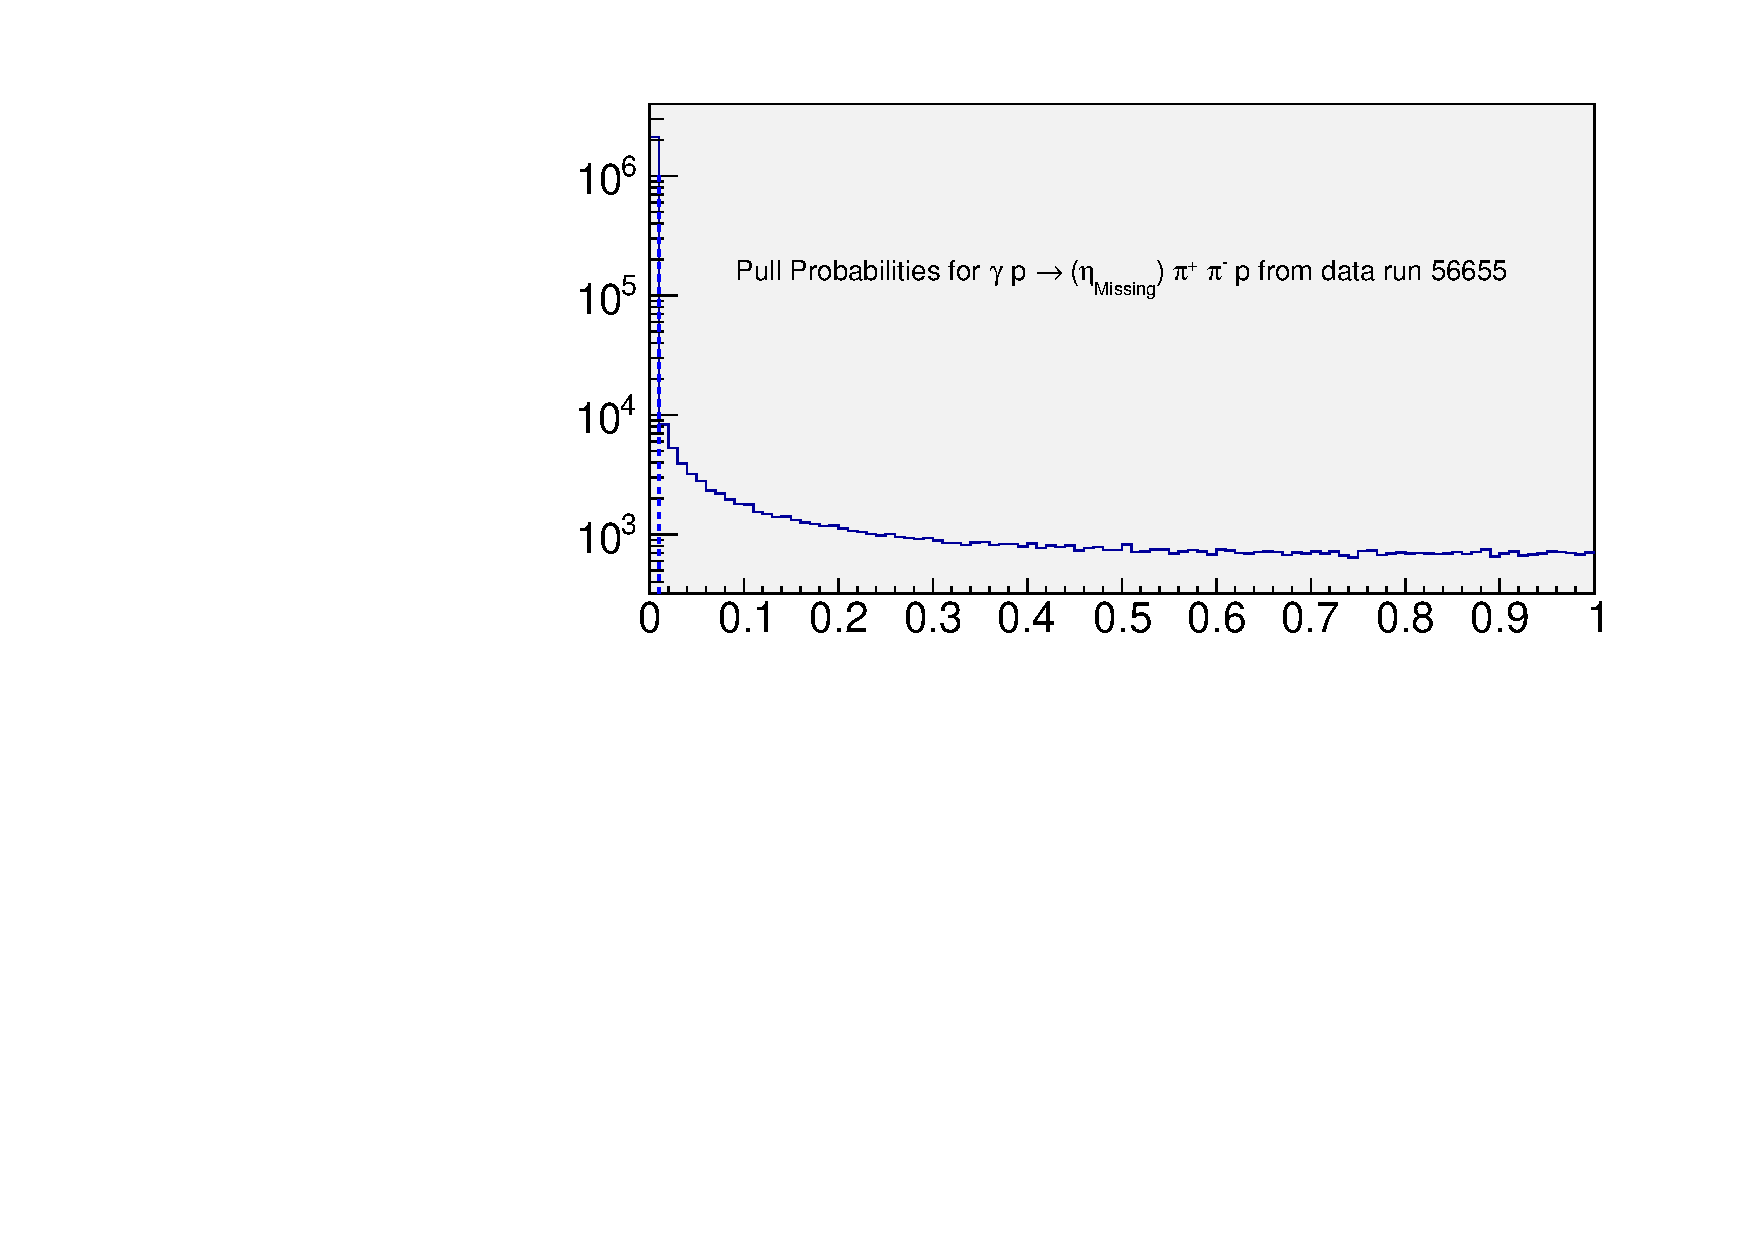
\includegraphics[width=12cm,height=8cm]{Prob_etafit.pdf}}
\caption{The Pull probability for a (1C) kinematic fit to $\gamma$ p $\rightarrow$ ($\eta_{Missing})$ $\pi^{+}$ $\pi^{-}$ p from data run 56655.}
\label{Fig5}
\end{figure} 

The tuned Kinematic fitter for the 4C constrained fit is again used for the channel below
\begin{eqnarray*}
\gamma p \rightarrow (\eta)_{Missing} \pi^{+} \pi^{-} p. (1C)
\end{eqnarray*}\\	
 The 1-C constrained fit requires the four-momentum [beam] + [target] - ( [$\pi^{+}$] [$\pi^{-}$] [p]) to be an [$\eta$] meson. The reaction hypothesis has the same set of final state particles as for the tuned channel, hence one can comfortably use it without tuning it for our reaction hypothesis again. The Pull probability for the channel is shown in Fig.~\ref{Fig5} and the dotted line at 0.01 shows the 1$\%$ Pull probability cut to reject events. 
\FloatBarrier
\subsection{$\mid$ $\cos\theta_{center-of-mass}$ of $\eta^{\prime}$ $\mid$ $\leq$ 0.85 Cut}
\label{Cos}


The events are generated with the differential cross sections of $\eta^{\prime}$ from the g11 measurement ~\cite{Williams:2009yj} within a $\mid$ $\cos\theta_{center-of-mass}$ of $\eta^{\prime}$ $\mid$ $\leq$ 0.85. The earlier measurement of CLAS g11 has reported the differential cross sections in $\mid$ $\cos\theta_{center-of-mass}$ of $\eta^{\prime}$ $\mid$ $\leq$ 0.85 window as the yield drops near to the beam pipe and hence this region is removed from the analysis.  

\subsection{$\mid$ $\cos\theta_{center-of-mass}$ of $\eta$ $\mid$ $\leq$ 0.85 Cut}
\label{CosEta}

  The $\eta$ mesons along the beam pipe in the forward and backward region is removed with a condition requiring $\mid$ $\cos$ $\theta_{center-of-mass}$ of $\eta$ $\mid$ $\leq$ 0.85.  The Figure.~\ref{Fig_CsE_1} shows the $\cos$($\theta$) distribution of $\eta$ meson in the rest frame of $\eta^{\prime}$ meson for both data and simulation. The Figure.~\ref{Fig_CsE_2} clearly shows the steep drop of acceptance for the $\eta$ meson with high kinetic energy decaying along the beam pipe region. Hence the a geometrical cut at $\mid$ $\cos$ $\theta_{center-of-mass}$ of $\eta$ $\mid$ $\leq$ 0.85 is placed in order to calculate integrated acceptance for Dalitz plot parameters. 
  
 \begin{figure}[ht!]
\centerline{
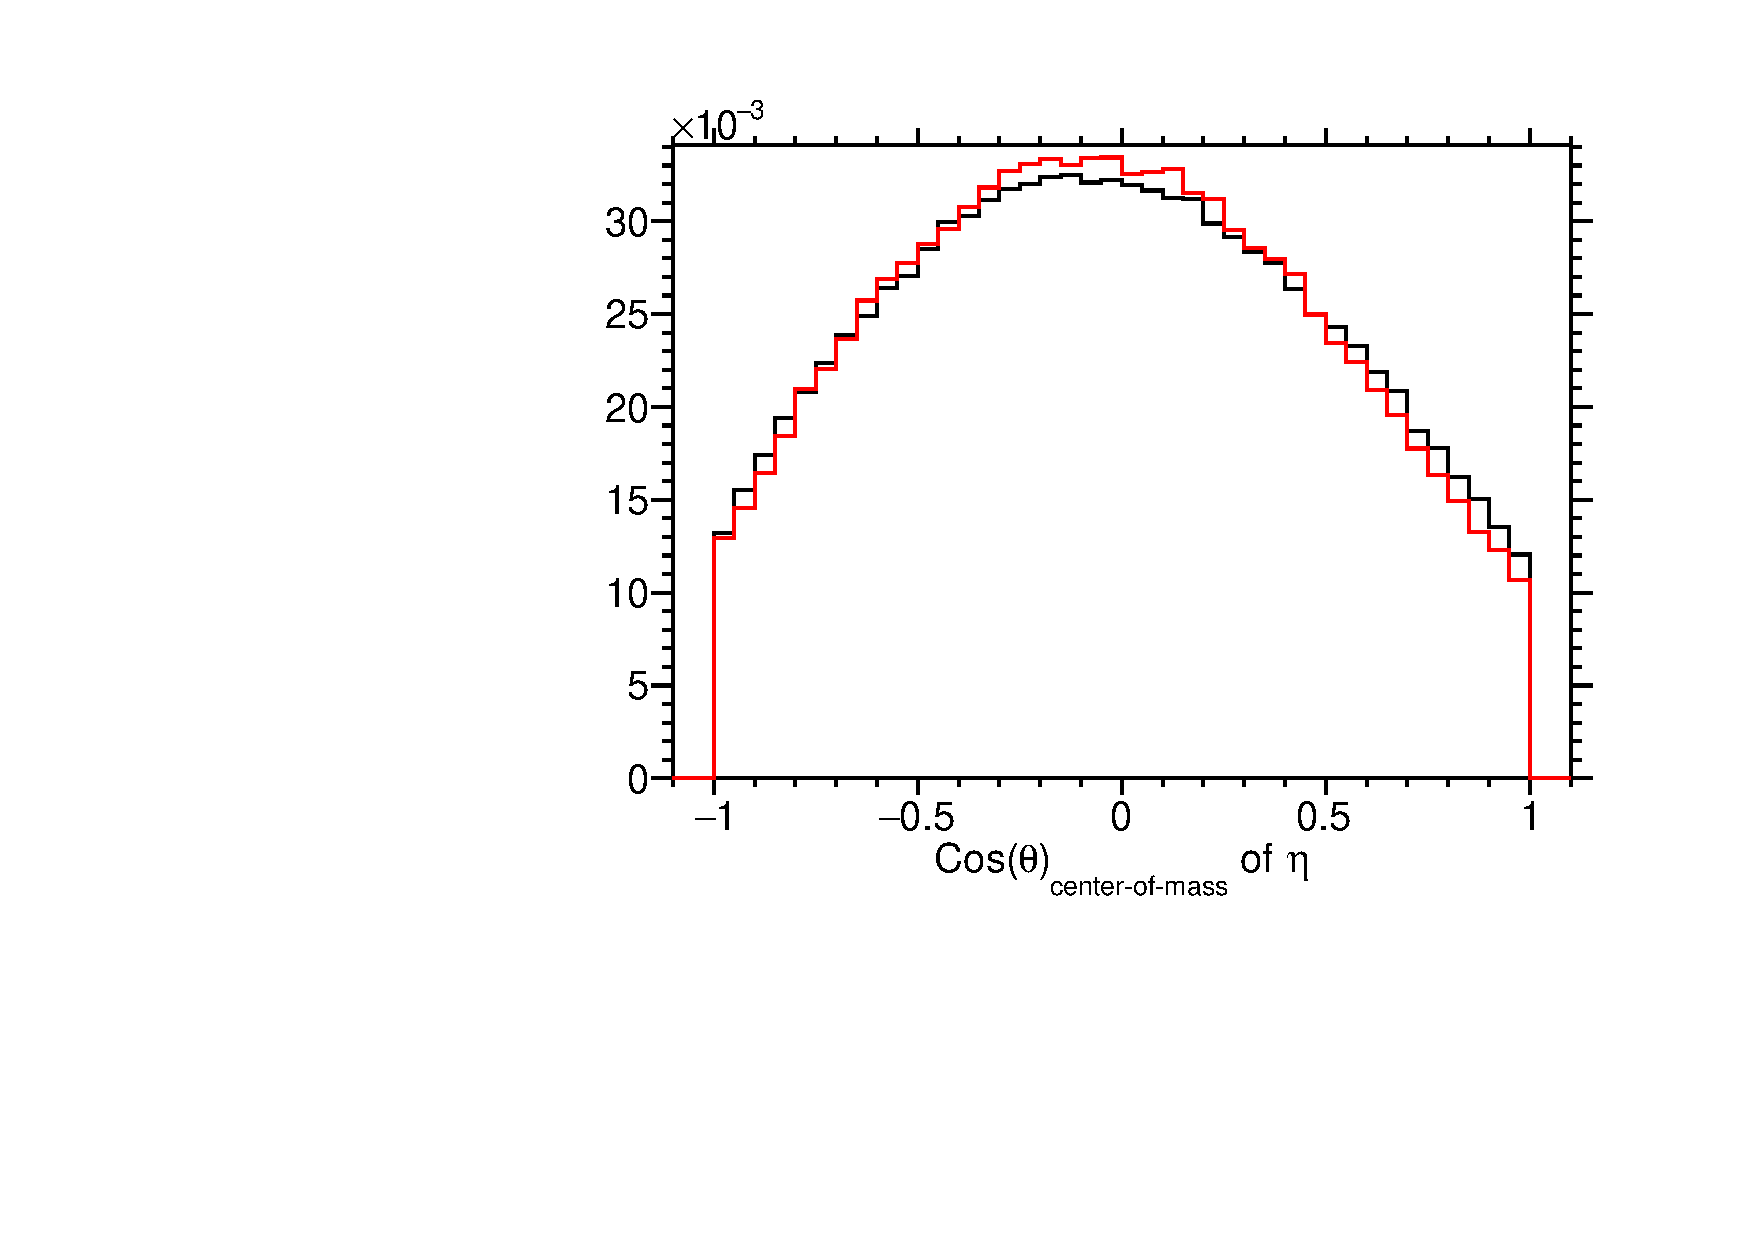
\includegraphics[width=12cm,height=8cm]{cs.pdf}}
\caption{$\cos\theta_{center-of-mass}$ of $\eta$ distribution from g12 data and simulation. }
\label{Fig_CsE_1}
\end{figure}


\begin{figure}[ht!]
\centerline{
%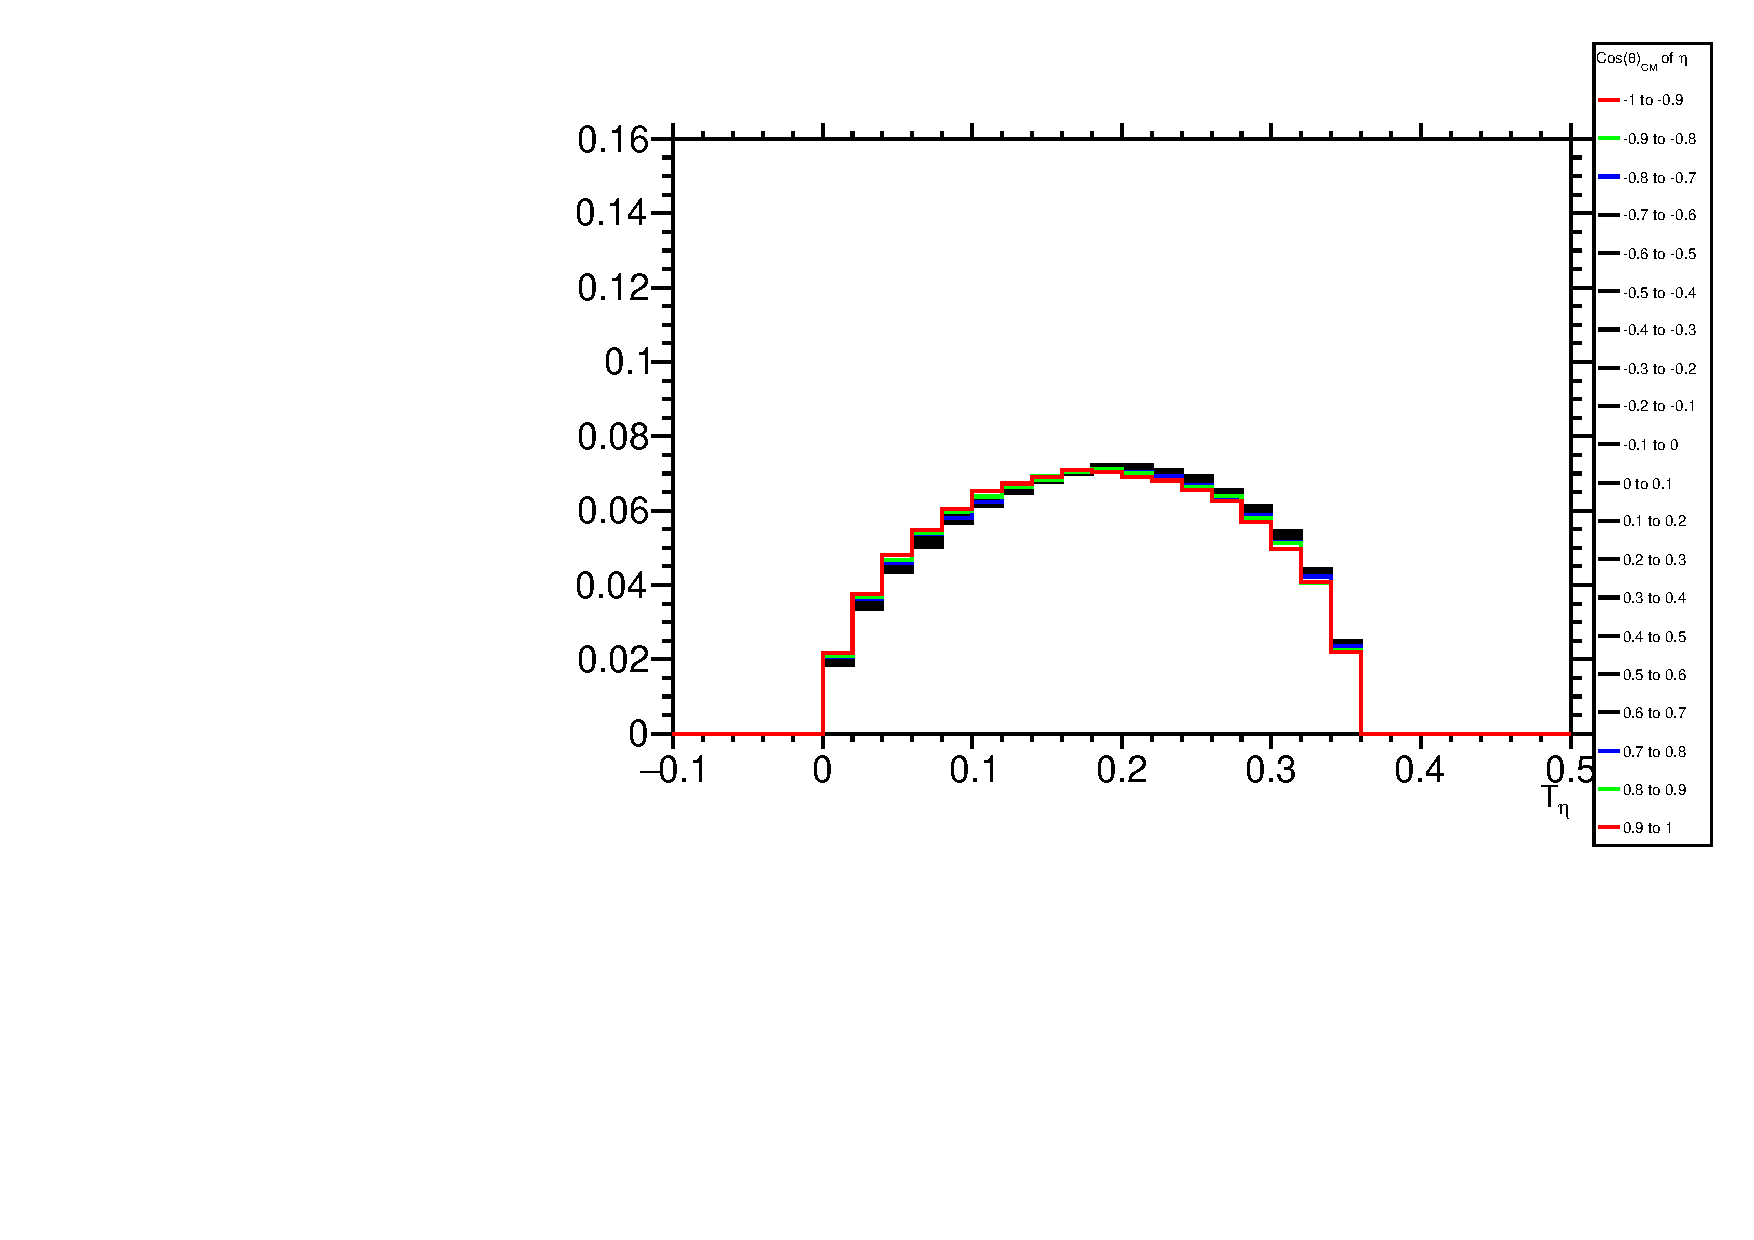
\includegraphics[width=12cm,height=8cm]{Gen_T.pdf}}
%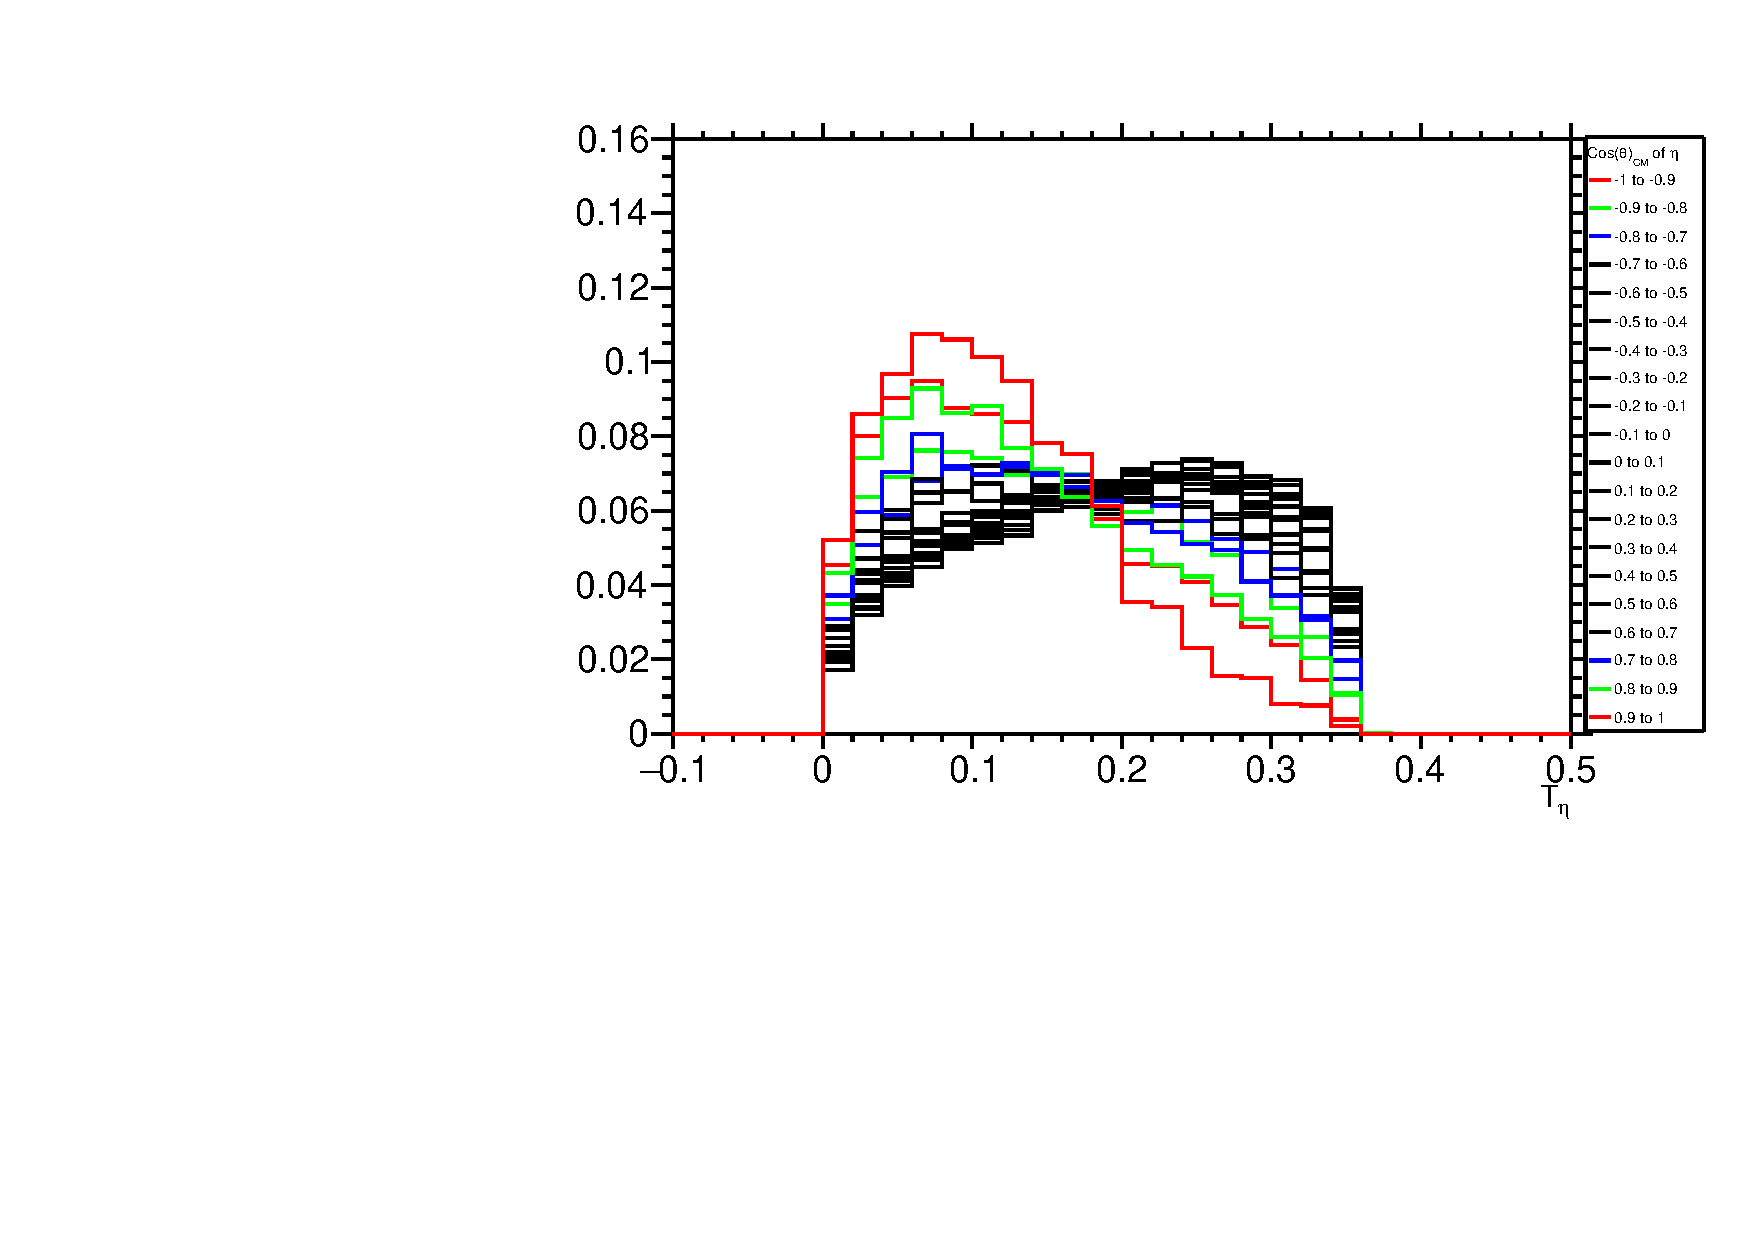
\includegraphics[width=12cm,height=8cm]{Sim_T.pdf}}
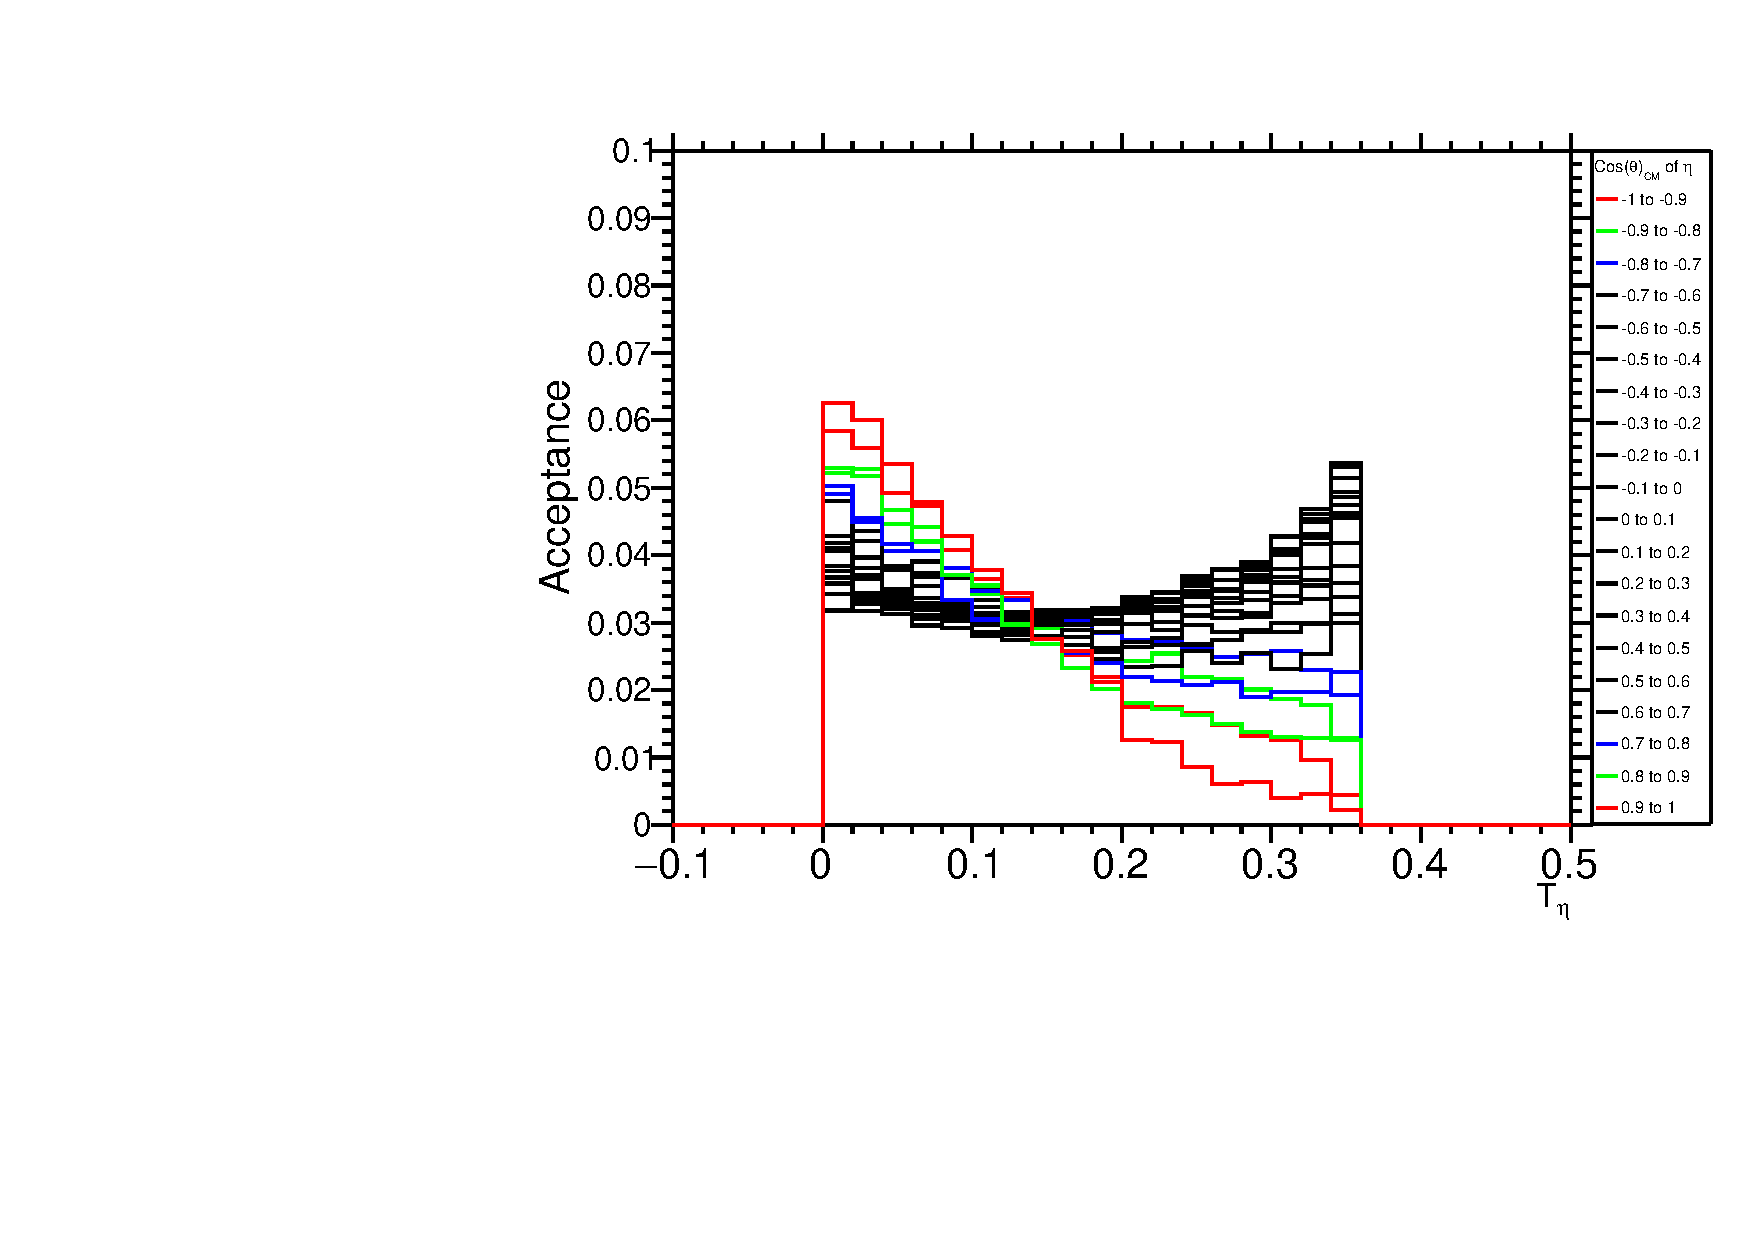
\includegraphics[width=12cm,height=8cm]{Acc_T.pdf}}
\caption{The acceptance vs $T_{\eta}$ in 0.1 bins of $\cos$ 
$\theta_{center-of-mass}$ of $\eta$ meson. }
\label{Fig_CsE_2}
\end{figure}

The kinematics of $\eta$ meson is directly related to the Dalitz variable Y. Hence a comparison of the cut is also presented for the Dalitz variable Y in Figure.~\ref{Fig_CsE_3} and  ~\ref{Fig_CsE_4} from simulation and g12 data respectively.    

\begin{figure}[ht!]
\centerline{
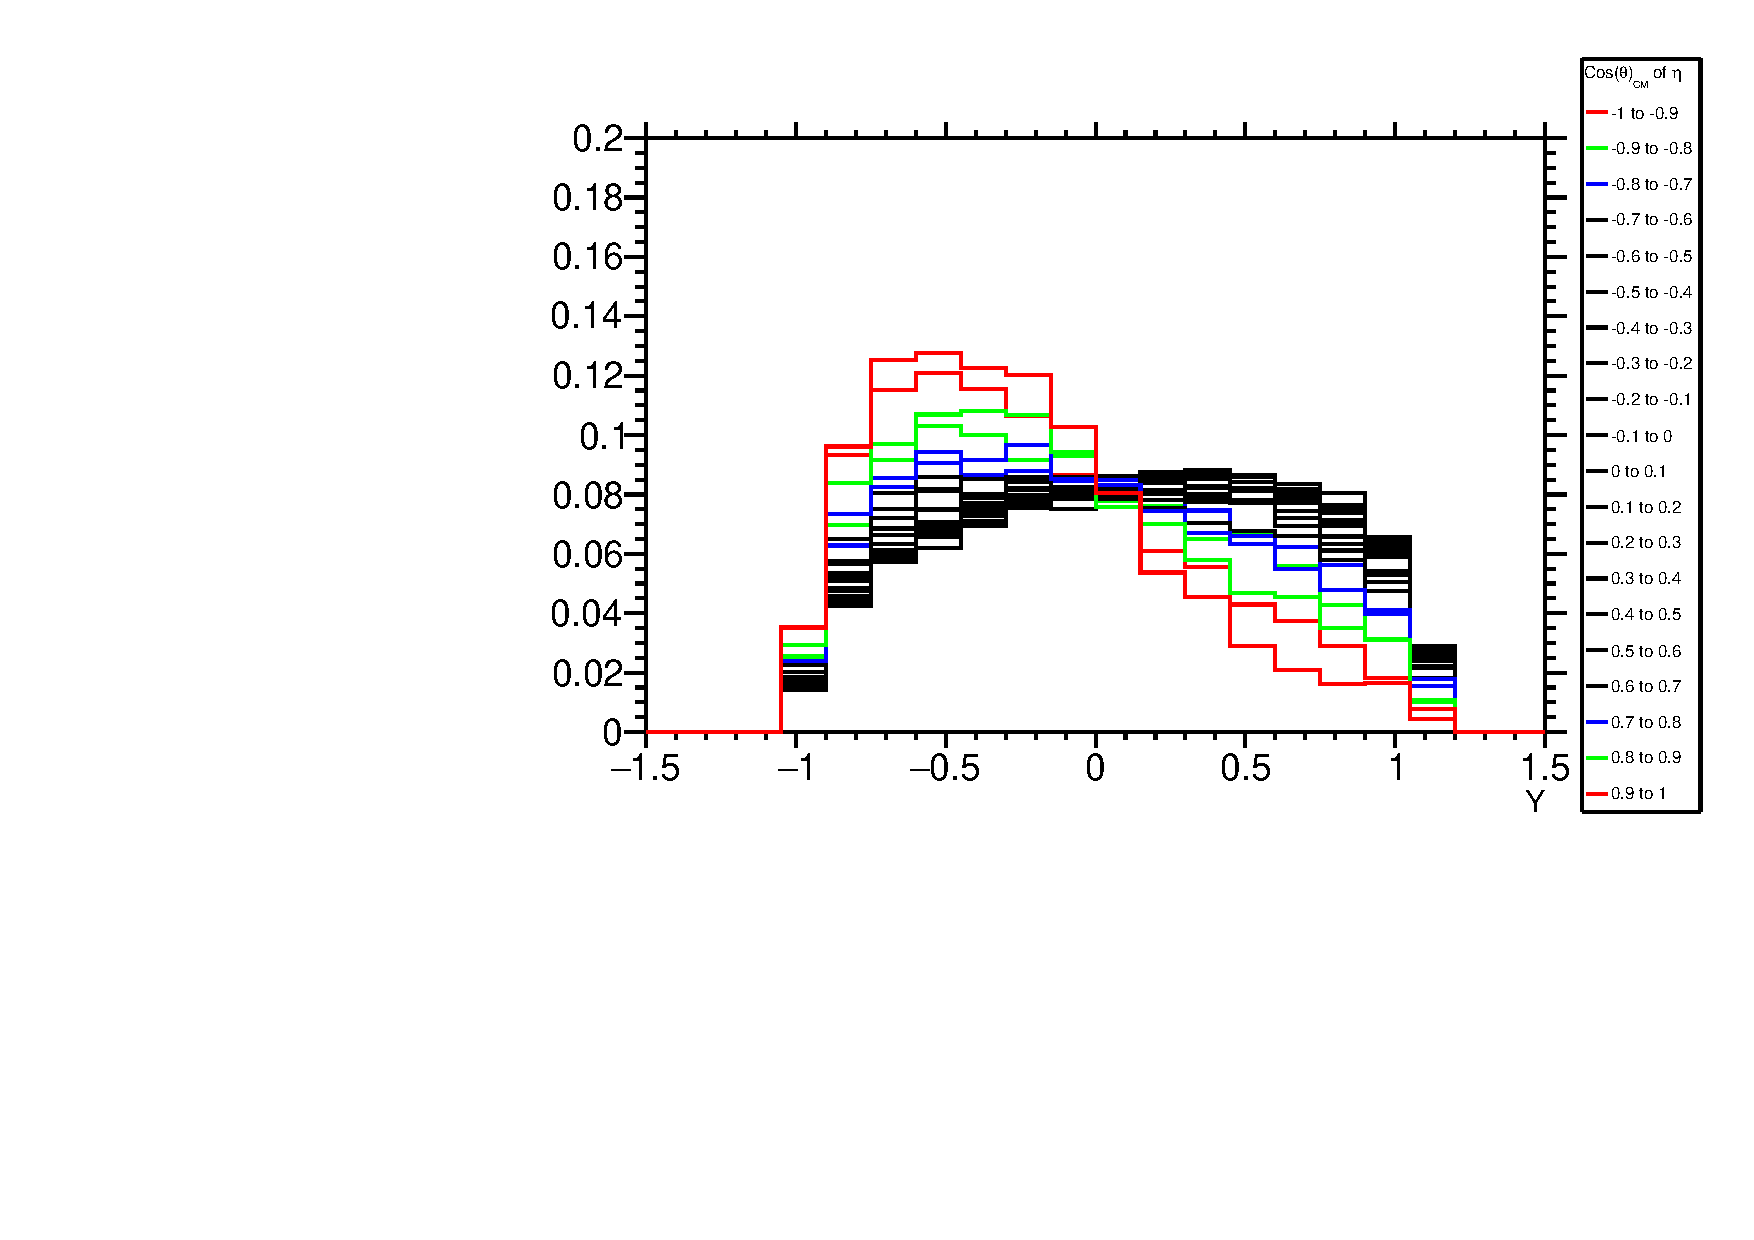
\includegraphics[width=12cm,height=8cm]{eta_CosTh_Cut.pdf}}
\caption{Dalitz Variable Y distribution normalised to 1 in each 0.1 bins of $\cos\theta_{center-of-mass}$ of $\eta$ from simulation.}
\label{Fig_CsE_3}
\end{figure}

\begin{figure}[ht!]
\centerline{
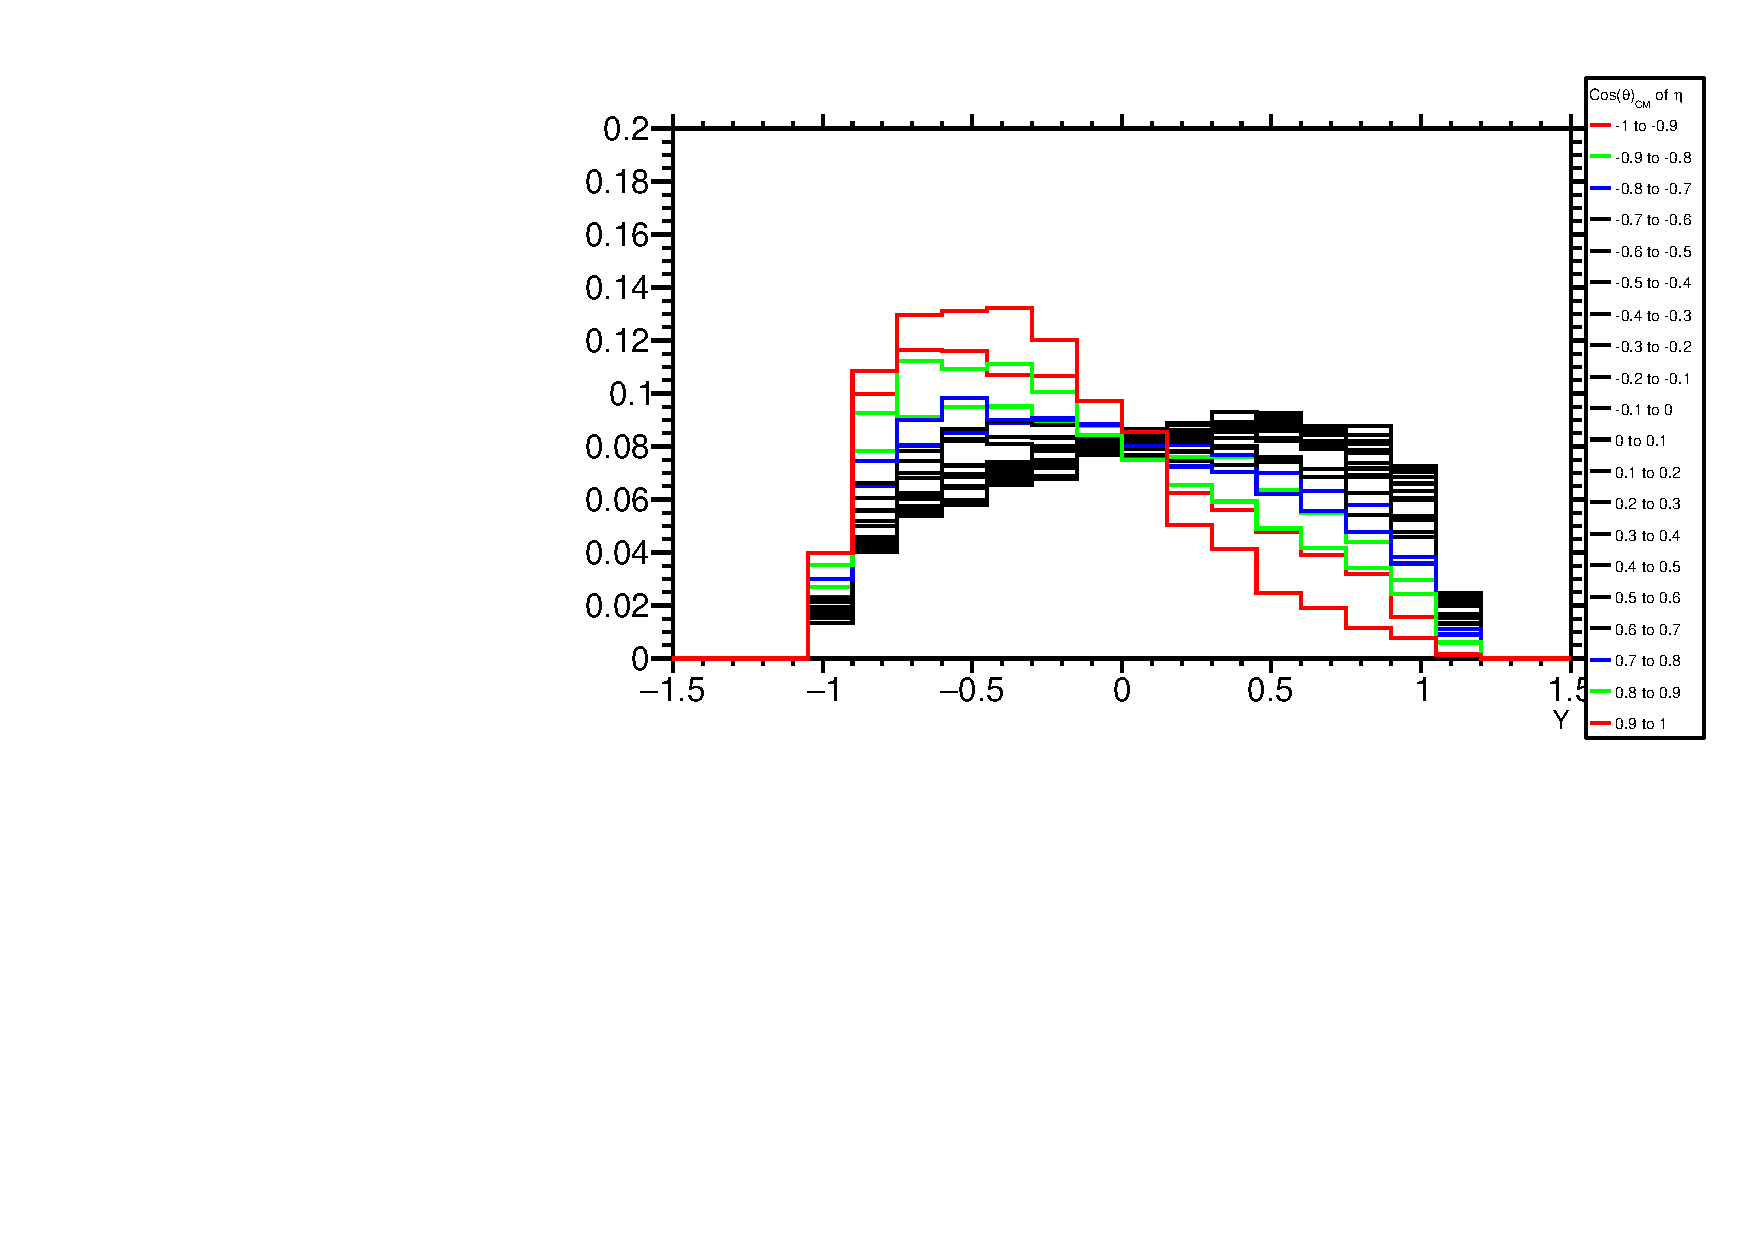
\includegraphics[width=12cm,height=8cm]{sim_CsEta.pdf}}
\caption{Dalitz Variable Y distribution normalised to 1 in each 0.1 bins of $\cos\theta_{center-of-mass}$ of $\eta$ from g12 data.}
\label{Fig_CsE_4}
\end{figure}
\FloatBarrier
\subsection{Vetex Cut}
\label{VCut}
In the g12 experiment the target was positioned -90 cm from the CLAS center. The target cell was 40 cm long and 2 cm in radius in the form of a cylinder filled with unpolarised liquid hydrogen. We used this target information and imposed it to all event vertexes. We required all events  production vertex tracks to originate in the target region via the condition that $\sqrt{v_{x}^{2} + v_{y}^{2}}$ $\leq$ 2 cm and -110 $\geq$ $v_{z}$ $\leq$ -70 cm. 

\begin{figure}[ht!]
\centerline{
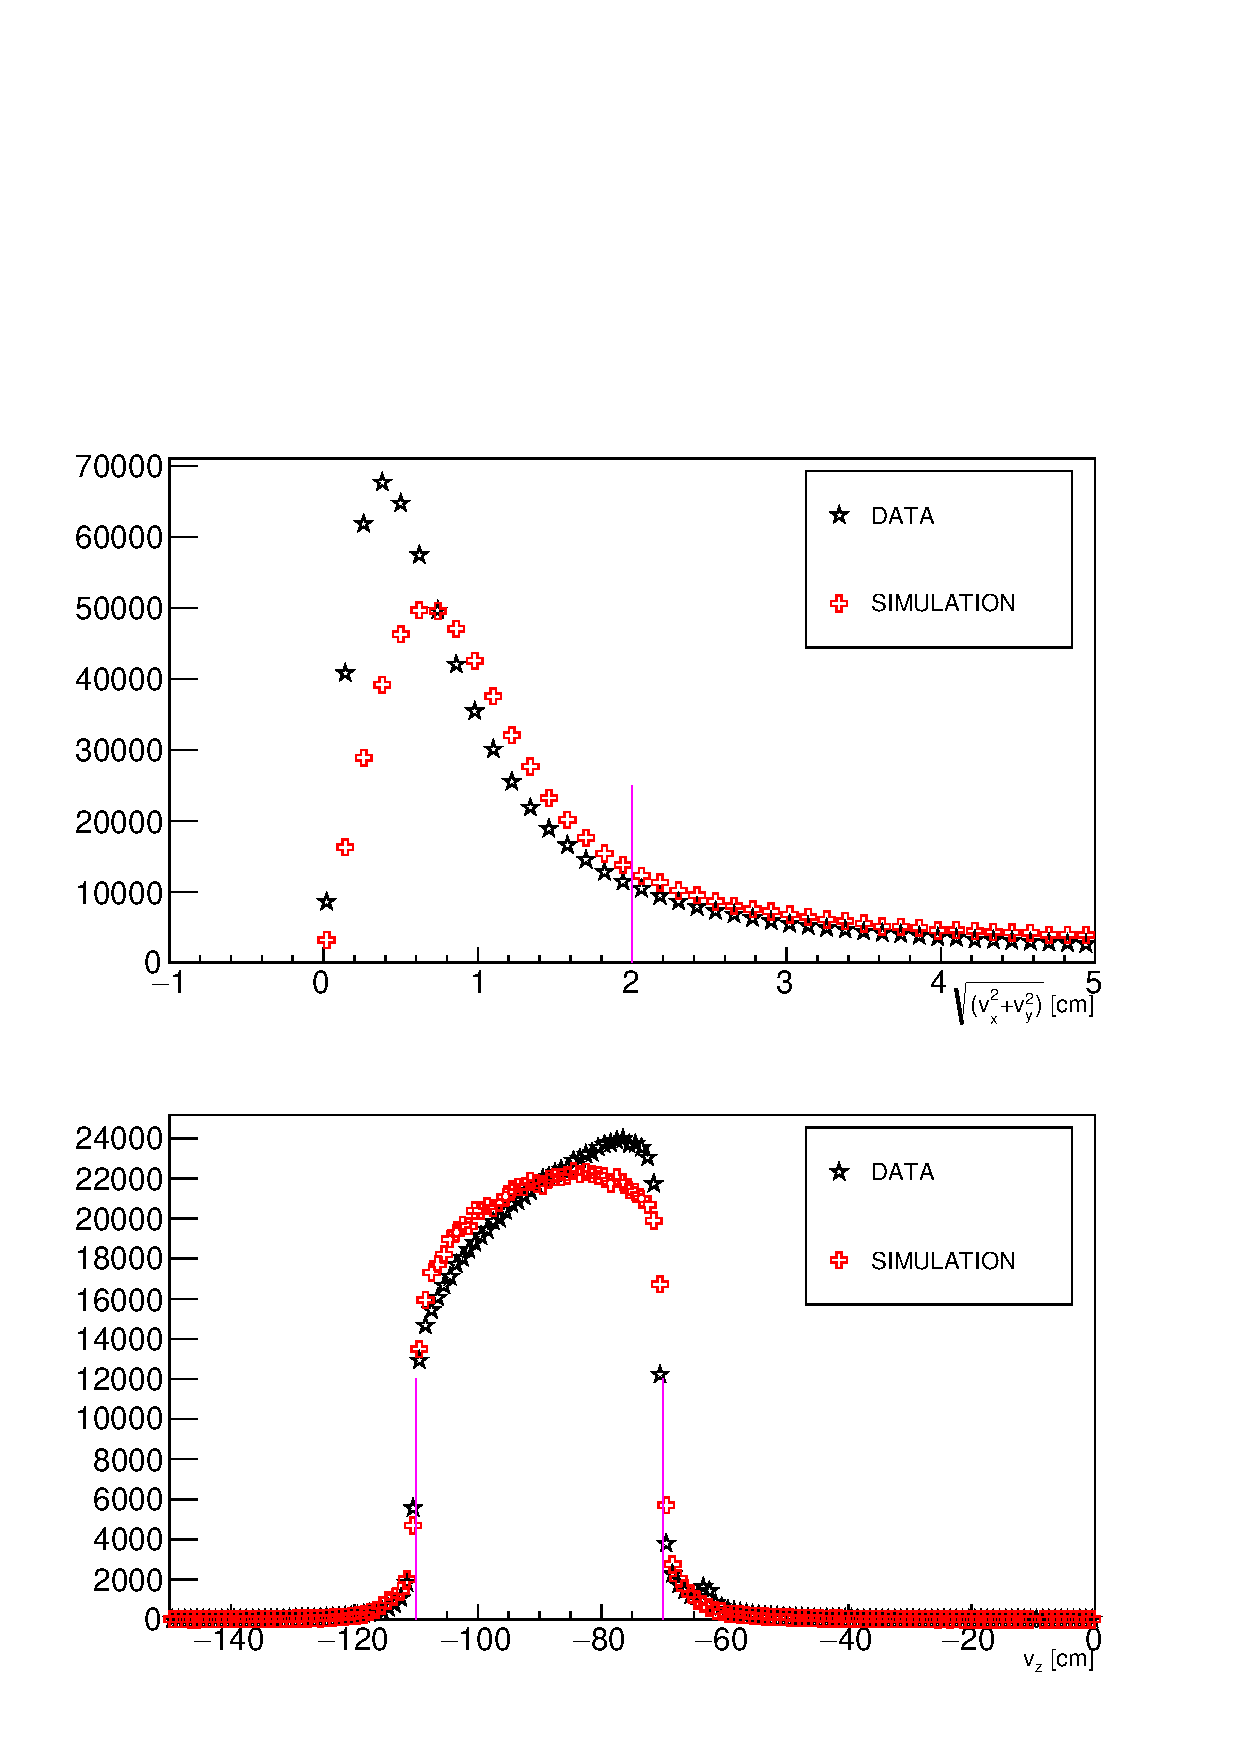
\includegraphics[height=5.8in]{vertex.pdf}}
\caption{[tpho + tprop -scvt] distribution from the simulation and data for proton, $\pi^{+}$ and $\pi^{-}$.}
\label{Fig1}
\end{figure}

\subsection{Timing Cuts on proton, $\pi^{+}$ and $\pi^{-}$}
\label{TCut}
As a post PID improvement of the detected final state particles $\pi^{+}$, $\pi^{-}$ and proton, we introduced a vertex timing $(t_{vert})$ cut of particles in the analysis. The $t_{vert}$, vertex time is the instant of time the particle left the target. One can calculate it through the information of the TOF detectors as,

\begin{eqnarray*}
t_{vert}(TOF) = t_{TOF}  -  \frac{l_{TOF}}{c\beta}
\end{eqnarray*}

where $t_{TOF}$ and $l_{TOF}$ are the measured time and length of particle in TOF sub detector. Here c is the velocity of light in vacuum and $\beta$ is the Lorentz factor of the particle calculated by knowing the velocity(v) of particle as $\beta = \frac{v}{c}$. The same vertex timing $(t_{vert})$ information can also be calculated from the RF-corrected time instant of the photon ($t_{photon}$)  crossing the target center measure by the tagger added with the $t_{prop}$, which is the propagation time from the center of the target to the track vertex. Given by,

\begin{eqnarray*}
t_{vert}(Tagger) = t_{photon} + t_{prop}.
\end{eqnarray*}


The difference of the $t_{vert}(TOF)$ from $t_{vert}(Tagger)$ is shown in Fig.$~\ref{Fig2}$, and we make a cut of $\pm$ 1.55 ns around 0 ns for all the final state particles in both simulation and data. 
\begin{figure}[ht!]
\centerline{
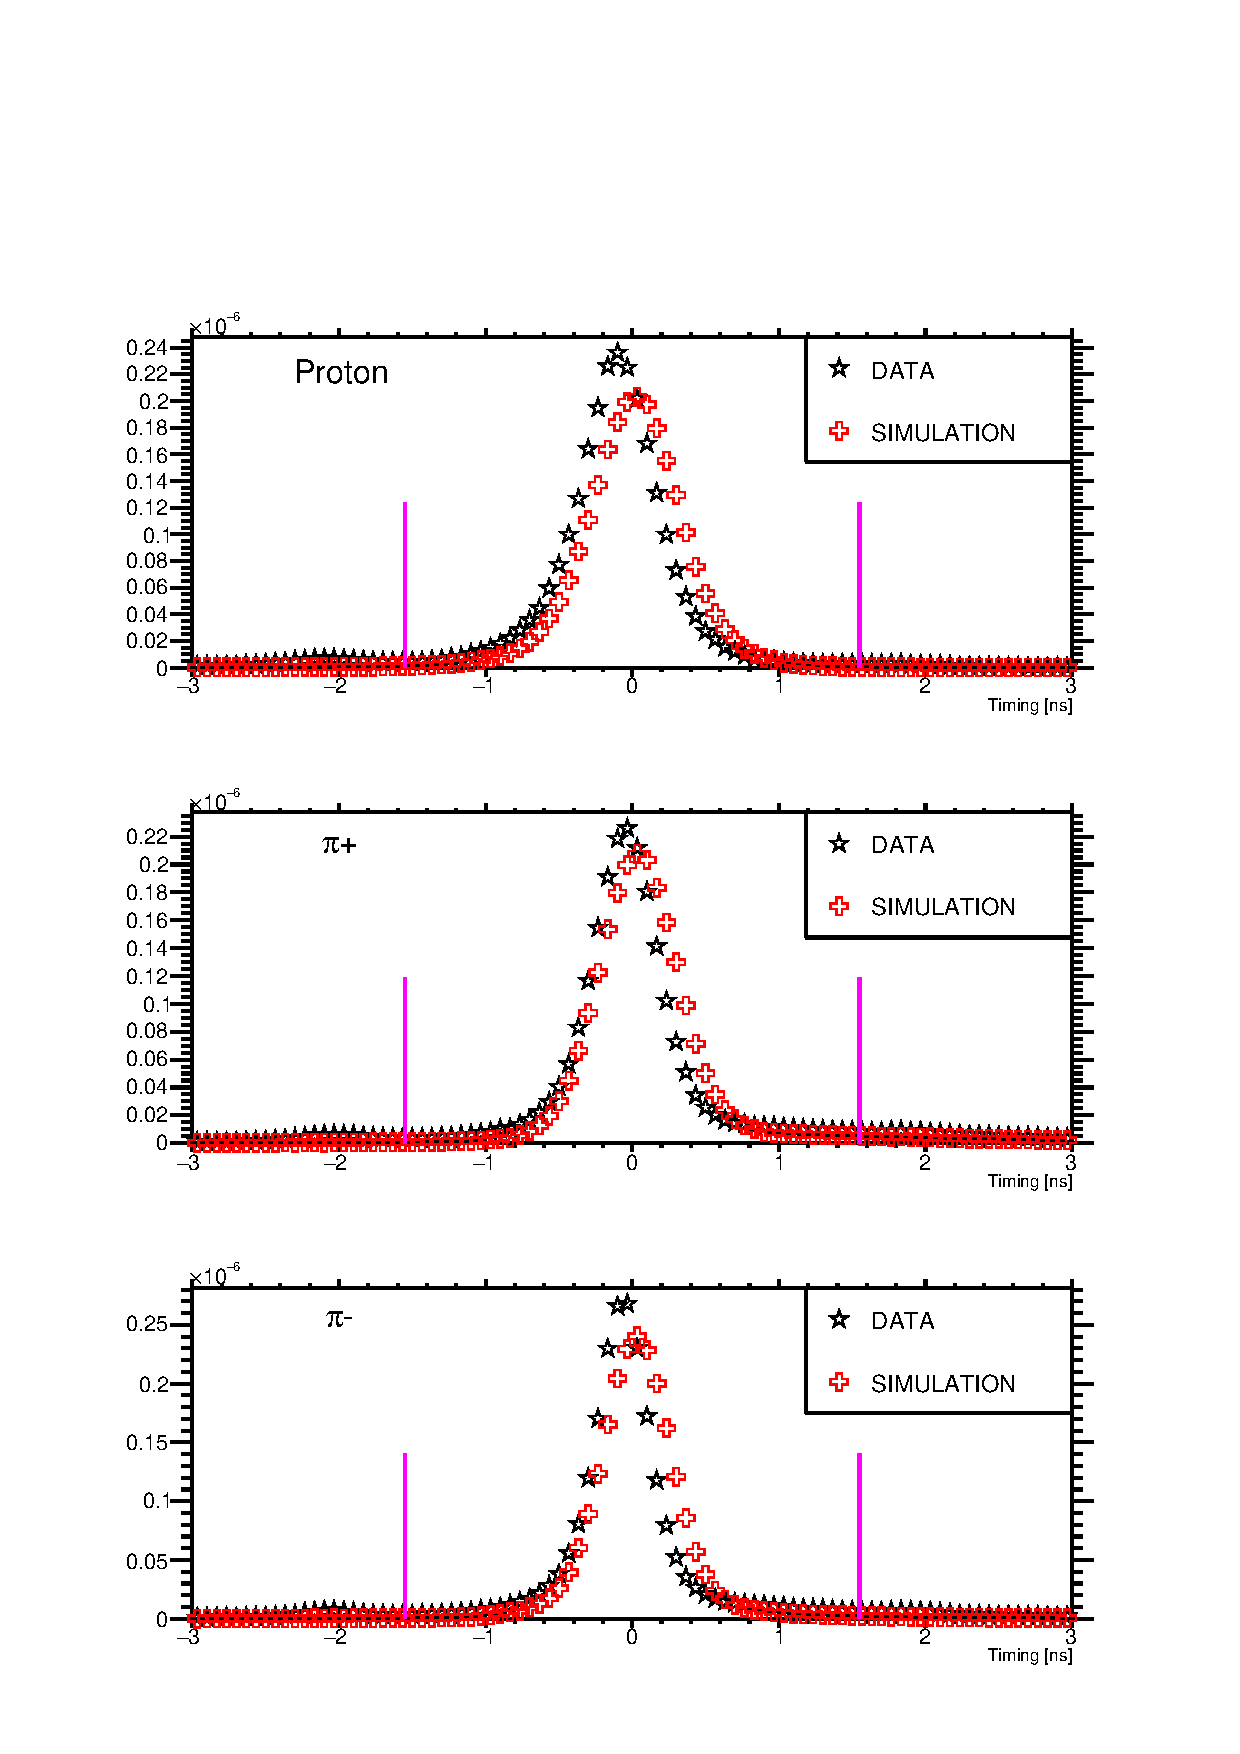
\includegraphics[height=7.8in]{timing.pdf}}
\caption{[$t_{vert}(TOF)$ - $t_{vert}(Tagger)$] distribution from the simulation and data for proton(Upper), $\pi^{+}$(Middle) and $\pi^{-}$(Lower).}
\label{Fig2}
\end{figure}
